\documentclass[12pt a4paper]{article}
\usepackage[utf8]{inputenc}
\usepackage[english] {babel}
\usepackage[letterpaper,top=2cm,bottom=2cm,left=3cm,right=3cm,marginparwidth=1.75cm]{geometry}
\usepackage{graphicx}
\usepackage[colorlinks=true, allcolors=blue]{hyperref}
\usepackage{pifont}
\usepackage{amsmath,amsthm,amsfonts}
\usepackage{latexsym,amssymb}
\usepackage{array}
\usepackage[T1]{fontenc}
\usepackage{natbib}
\newtheorem{teor}{Teorema}
\title{GEOMETRÍA}
\author{Jecer David Quito Huanca}
\begin{document}
\maketitle
\section{Axiomas Sobre la Medición de Ángulos}
Los axiomas sobre la medición de ángulos son declaraciones básicas que establecen las reglas fundamentales para la comparación y manipulación de las medidas de los ángulos en geometría. Estos axiomas proporcionan la base sobre la cual se construye todo el estudio de los ángulos y sus propiedades. Incluyen afirmaciones sobre la igualdad de medidas de ángulos, la suma de ángulos en diferentes configuraciones geométricas, y la definición de ángulos estándar, como los ángulos rectos, agudos y obtusos. Estos axiomas son esenciales para comprender y trabajar con ángulos en contextos matemáticos y científicos, ya que establecen las reglas fundamentales que gobiernan su comportamiento y relación en el espacio euclidiano.
\subsection{Definicion}
\begin{itemize}
    \item Definición 3.1 Llamamos ángulo a la figura formada por dos
líneas semirrectas con el mismo origen.
\begin{center}
    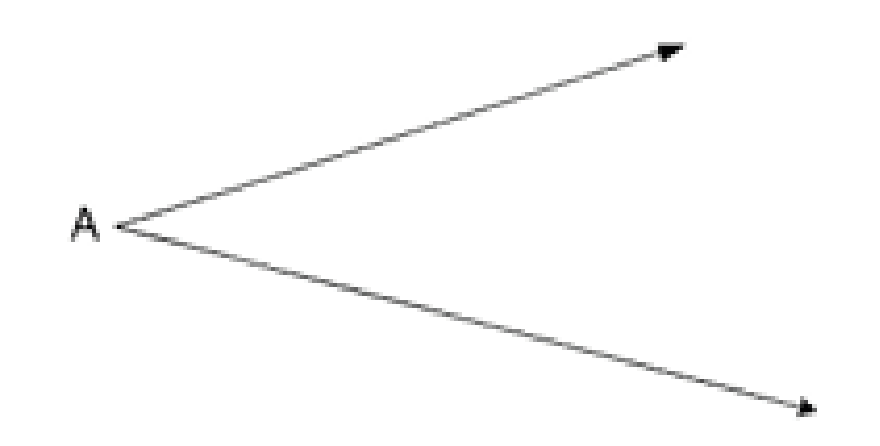
\includegraphics[scale=0.8]{p.png}
\end{center}
    \item Definición 3.2 Diremos que una media línea divide un semiplano
si está contenido en el semiplano y su origen es un punto en el
línea que lo determina.
    \item Definición 3.4 Se dice que dos ángulos son suplementarios si la suma
de sus medidas es 180°. El suplemento de un ángulo es el ángulo.
adyacente al ángulo dado obtenido prolongando uno de sus
lados.
\begin{center}
    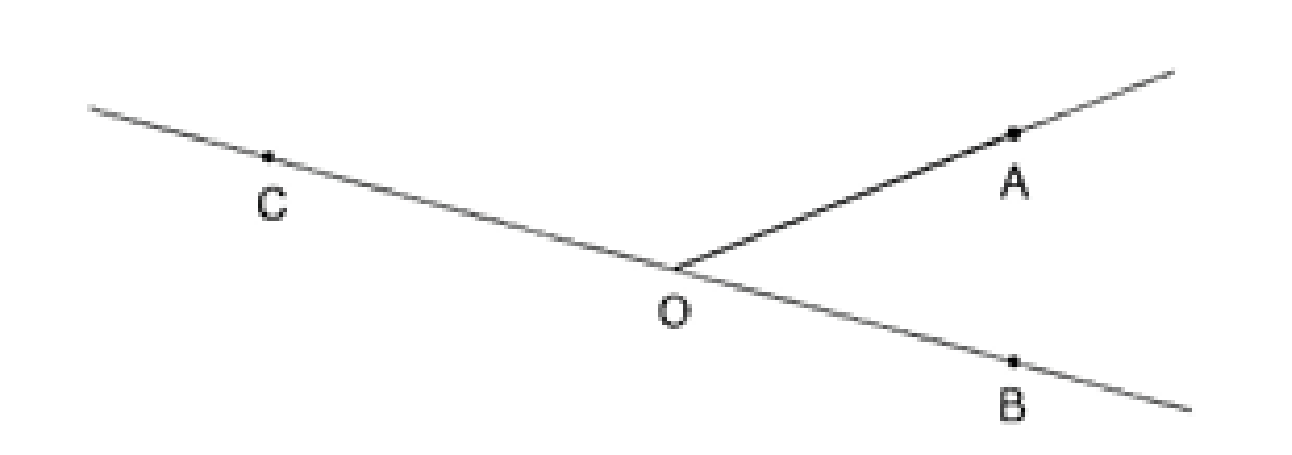
\includegraphics[scale=0.8]{r.png}
\end{center}
    \item Definición 3.6 Un ángulo cuya medida es 90° se llama ángulo
derecho. Está claro que el suplemento de un ángulo recto también es un
ángulo recto. Cuando dos líneas rectas se cruzan, si un enlace de cuatro
ángulos formados por ellos es recto, entonces todos los demás también son
ellos estarán. En este caso diremos que las rectas son perpendiculares.

\end{itemize}

\begin{center}
    \begin{tabular}{|m{3cm}|m{10cm}|}\hline
\bf Axioma & \bf Concepto \\
\hline
Axioma III(4) & Todo ángulo tiene una medida mayor o igual a cero.
La medida de un ángulo es cero si y sólo si consta de
dos rayos coincidentes. \\
\hline
Axioma III(5) & Es posible colocar, en correspondencia uno a uno, los números reales entre cero y 180° y semi-rectas del mismo origen que dividen un semi-plano dado, de modo que la diferencia entre. Estos números son la medida del ángulo formado por las medias líneas correspondiente. \\
\hline
Axioma III(6) & Si un semi-recta Soc divide un ángulo AÔB, entonces.
AÔB = AÔC + CÔB \\
\hline
\end{tabular}
\end{center}
\section{Teorema}
\begin{teor}\label{uno}
Por cualquier punto de una recta pasa una única perpendicular a esta línea.
\begin{proof}[Demostracion]
(Existencia). Dada una recta m y un punto A sobre ella, la
dos semi-rectas determinados por A forman un ángulo agudo. Considere un enlace de semi-plano determinado por la recta m. De acuerdo con el axioma III(5), entre todos las semi-rectas con origen A, que dividen el semi-plano fijo, hay uno cuya coordenada será la
número 90. Este rayo se forma, con los dos semi-rectas determinados
nada por el punto A en la recta m, ángulo de 90°. Por lo tanto ella es
perpendicular a la recta m.

(Singularidad). Supongamos que hubiera dos líneas rectas ${n}$ y ${n}'$ pasando por el punto A y perpendicular a m. Adjuntar un semi-plano determinado por m. Las intersecciones son rectas ${n}$ y ${n}'$ con este semi-plano son semi-rectas que forman un ángulo 
$\alpha$ y,
\begin{center}
    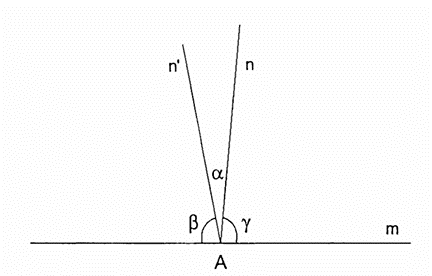
\includegraphics[scale=0.8]{Imagen1.png}
\end{center}
como en la figura, forma otros dos ángulos $\beta$ y $\gamma$ con las semi-rectas
determinadas por el punto A en la recta m.

Como n y {n}' son perpendiculares a m entonces 
\begin{center}
    $\beta=\gamma=90$
\end{center}
Por otro lado, debemos tener 
\begin{center}
    $\alpha+\beta+\gamma=180$
\end{center}
Luego
\begin{center}
    $\alpha=0$
\end{center}
 y las rectas ${n}$ y ${n}'$ coinciden.

\end{proof}
\end{teor}

\bibliographystyle{plain}
\bibliography{References}
Geometria euclidiana plana
Volumen 11 de Coleção do Professor de Matemática
Autor	João Lucas Marques Barbosa
Edición	9
Editor	Sociedade Brasileira de Matemática, 2012
ISBN	8585818026, 9788585818029
N.º de páginas	222 páginas |1|

\end{document}
